% !TEX TS-program = latex  
\documentclass[english,dvipsnames]{beamer}     %  ,handout
\usepackage[activeacute,spanish]{babel}
\usepackage{babel}
\usepackage[utf8]{inputenc}
\usepackage{pgffor} 
\usepackage{listings}
\usepackage{graphicx}
\usepackage{multirow}
\usepackage{algorithm}
\usepackage{algorithmic}
\usepackage{color, colortbl}
\usepackage[absolute,overlay]{textpos}
\usepackage{ bbold }
\usepackage[
  style=numeric,
  %autocite=footnote,
  maxnames=10,
  babel=hyphen,
  hyperref=true,
  abbreviate=false,
  backend=biber,
  doi=false,
  url=false,
  giveninits=true,
  isbn=false,
  indexing=true
  ]{biblatex}   

  \renewcommand{\algorithmicrequire}{\textbf{Input:}}
  \renewcommand{\algorithmicensure}{\textbf{Output:}} 
  \resetcounteronoverlays{algorithm}

\usepackage{standalone}
  \standaloneconfig{mode=image} % mode=buildnew OR mode=image %%%%%

\usepackage[T1]{fontenc}
\usepackage{multicol}
\usepackage{textcomp} % to get the right copyright, etc.
\usepackage{amsmath} % before lucidabr
\usepackage{tikz}
\usepackage{pgfplots} 
  \usetikzlibrary{patterns}
  \usetikzlibrary{snakes}
\usetikzlibrary{shapes,arrows,decorations.markings}
\usetikzlibrary{positioning}
\usetikzlibrary{calc}
%\usetikzlibrary{shapes,arrows}


\setlength{\parskip}{0pt}%
\usepackage{soul}
\usepackage{movie15}
\usepackage{smartdiagram}

% use Lucida fonts for both text and math.
% \usepackage[T1,altbullet,expert,nofontinfo,lucidascale]{lucidabr}     % get larger bullet
\pgfplotsset{select coords between index/.style 2 args={
    x filter/.code={
        \ifnum\coordindex<#1\def\pgfmathresult{}\fi
        \ifnum\coordindex>#2\def\pgfmathresult{}\fi
    }
}}

\DeclareEncodingSubset{TS1}{hlh}{1}  % including \oldstylenums
%%%%%
\addtobeamertemplate{footnote}{\vspace{-6pt}\advance\hsize-0.5cm}{\vspace{6pt}}
\makeatletter
\renewcommand*{\footnoterule}{\kern -3pt \hrule \@width 2in \kern 8.6pt}

\usetheme{Madrid}  % default minimalista

\usecolortheme{rose}

\newenvironment<>{problock}[1]{%
  \begin{actionenv}#2%
      \def\insertblocktitle{#1}%
      \par%
      \mode<presentation>{%
        \setbeamercolor{block title}{fg=white,bg=orange!20!black}
       \setbeamercolor{block body}{fg=black,bg=olive!50}
       \setbeamercolor{itemize item}{fg=orange!20!black}
       \setbeamertemplate{itemize item}[triangle]
     }%
      \usebeamertemplate{block begin}}
    {\par\usebeamertemplate{block end}\end{actionenv}}





%\bibliographystyle{apalike}
\DefineBibliographyStrings{english}{%
  bibliography = {References},
}
\addbibresource{biblio.bib}
%\bibliography{biblio}
\renewcommand{\footnotesize}{\scriptsize}
%----------------------------------------------------------------------------%
\title[Efecto del Fe en el pCO$_2$]{Contribución oceánica regional de la fertilización con hierro a los cambios de CO$_2$ atmosférico desde el Último Máximo Glacial hasta el Holoceno}

\author[Natalia Opazo C.]{Natalia Opazo Cuevas}
 
\date{\tiny{2 mayo 2019}}
\institute[PUC]{Pontificia Universidad Católica de Chile} 
\subject{Departamento de Geografía}
\AtEveryCitekey{\iffootnote{\color{red}\scriptsize}{\color{blue}}}

%\usebackgroundtemplate{\includegraphics[width= \paperwidth, height=\paperheight]{./imagenes/back.jpg}}
\beamertemplatenavigationsymbolsempty
\begin{document}

\tikzstyle{decision} = [diamond, draw, fill=purple!20, 
    text width=4.5em, text badly centered, node distance=3cm, inner sep=0pt]
\tikzstyle{block} = [rectangle, draw, fill=blue!20, 
    text width=5em, text centered, rounded corners, minimum height=4em]
\tikzstyle{blockn} = [rectangle, draw, fill=purple!20, 
    text width=5em, text centered, rounded corners, minimum height=4em]    
\tikzstyle{line} = [draw, -latex']
\tikzstyle{cloud} = [draw, ellipse,fill=red!20, node distance=3cm,
    minimum height=2em]

\begin{frame}
  \begin{center}
 \includegraphics[height=2.5cm]{./imagenes/LogoUC(COLOR).jpg}
  \end{center}
  \titlepage
\end{frame}

%%%%%%%%%%%%%%%%%%%%%%%%%%%%%%55
%\usebackgroundtemplate{}
\begin{frame}{Contenidos}
\begin{block}
\centering
\
\vspace{10pt}
\tableofcontents[pausesections]
\vspace{10pt}
\end{block}
\end{frame}

%%%%%%%%%%%%%%%%%%%%%%%%%%%%%%%%%%
\section{Introducción}
\begin{frame}{Planteamiento del problema}
\begin{minipage}[b]{0.3\textwidth}
\begin{block}{}
\small{
\begin{itemize}
\uncover<1->{\item{} \scriptsize{La tierra ha pasado por periodos fríos (\alert{glaciales}) y periodos cálidos (\alert{interglaciales}).}

\uncover<1->{\item{} La concentración de pCO$_2$ atmosférico en los últimos 800000 años ha variado entre $\sim$ \alert{180 - 280 ppm}.}

\only<2-4>{\item{} En octubre del 2017 se alcansó una concentración atmosférica de CO$_2$ de \alert{403.3 ppm}.}} 
\end{itemize}}
\end{block}
\end{minipage}\quad{\only<1>{
\begin{minipage}[t]{0.65\textwidth}%
\centering
\includegraphics[width=0.95\textwidth,height=0.6\textheight]{./imagenes/CO2_DUST.png}
\end{minipage}}
 \only<2>{
\begin{minipage}[t]{0.6\textwidth} 
%\begin{minipage}{0.7\textwidth}
\centering
\pgfplotstableread{./plot/CO2.txt} 
\datatable% 
%%%%%%%%%%%%%%%%%%%%%%
\resizebox*{!}{.7\textheight}{
  \begin{tikzpicture}[scale=1]
  \begin{axis}[
     % title={Temperature dependence of CuSO$_4\cdot$5H$_2$O solubility},
      xlabel={Años},
      ylabel={Concentración de pCO$_2$},
      xmin=1950, xmax=2010,
      ymin=310, ymax=400,
      xtick={1950,1960,1970,1980,1990,2000,2010},
      ytick={310,320,330,340,350,360,370,380,390,400},
      %legend pos=north west,
      ymajorgrids=true,
      grid style=dashed, 
  ]
  \addplot[
     color=red,
     mark=square,
      ] table[x=Ano,y=CO2] from \datatable;
  %%     }
  %%  }
     % \legend{CuSO$_4\cdot$5H$_2$O} \includegraphics[width=\textwidth]{./imagenes/CO2ani.jpg}
    \end{axis}
    \node[] at (5.5, 1)    {\includegraphics[width=0.25\textwidth]{./imagenes/CO2ani.jpg}};
  \end{tikzpicture}
}
%%%%%%%%%%%%%%%%%%%%%%%
\end{minipage}} \hfil
\only<3>{
\begin{minipage}[t]{0.6\textwidth}
\centering
    \includegraphics[height=.7\textheight]{./imagenes/noticia.png}
\end{minipage}}
\only<4>{
\begin{minipage}[t]{0.6\textwidth}
\centering
    \includegraphics[height=.7\textheight]{./tikz/smartdiag}
\end{minipage}}}
\end{frame}


%%subsection{Polvo}
%%\begin{frame}{Polvo}
%%\begin{minipage}{0.9\textwidth}
%%\centering{
%%\begin{minipage}{0.4\textwidth}
%%\centering
%%    \includegraphics[width=\textwidth]{./imagenes/%%dust2_pag97book.pdf}
%%\end{minipage}
%%
%%\begin{minipage}{\textwidth}
%%\begin{center}
%%\begin{block}{}
%%
%%\begin{itemize}
%%\item{} \tiny{El \alert{polvo eólico} es una de las %%principales \alert{fuentes de hierro para el océano} %%abierto.}
%%\item{} \tiny{El polvo es producto de la erosión eólica.}
%%\item{} \tiny{Los mecanismos que lo llevan a cabo son: }
%%\begin{itemize}
%%\item{} \tiny{Arrastre aerodinámico}
%%\item{} \tiny{Saltación}
%%\item{} \tiny{Degradación de granos}
%%\end{itemize}
%%\item{} \tiny{Sólo una fracción del orden 10$^-6$ se %%convertirá en un flujo vertical (polvo suspendido en la %%atmósfera) \cite{marticorena1997factors}}
%%\end{itemize}
%%
%%\tiny{\alert{¿Pero qué relación tiene el polvo con el %%dióxido de carbono?}}
%%\end{block}
%%\end{center}
%%\end{minipage}}
%%
%%\end{minipage}
%%\end{frame}

%%%%%%%%%%%%%%%%%%%%%%%%%%%%%%%
\subsection*{Bomba biológica}

\begin{frame}{Bomba biológica orgánica}
\centering
    \includegraphics[width=0.9\textwidth,height=0.89\textheight]{./imagenes/bomba.pdf}
%\end{minipage} }
\end{frame}

%%%%%%%%%%%%%%%%%%%%%%%%%%%%%%%%%

\begin{frame}{Zonas HNLC}
    \begin{center}

    \begin{minipage}{0.9\textwidth}
    \begin{block}{}
 \begin{itemize}
  \uncover<1->{\item{} \scriptsize{Zonas limitadas por Fe.} }
  \uncover<2->{\item{} \scriptsize{Tienen alto contenido de nutrientes y bajas concentraciones de clorofila.}} 
\end{itemize}
    \end{block}
    \end{minipage}
       
\uncover<1-2>{\begin{minipage}{0.9\textwidth}
    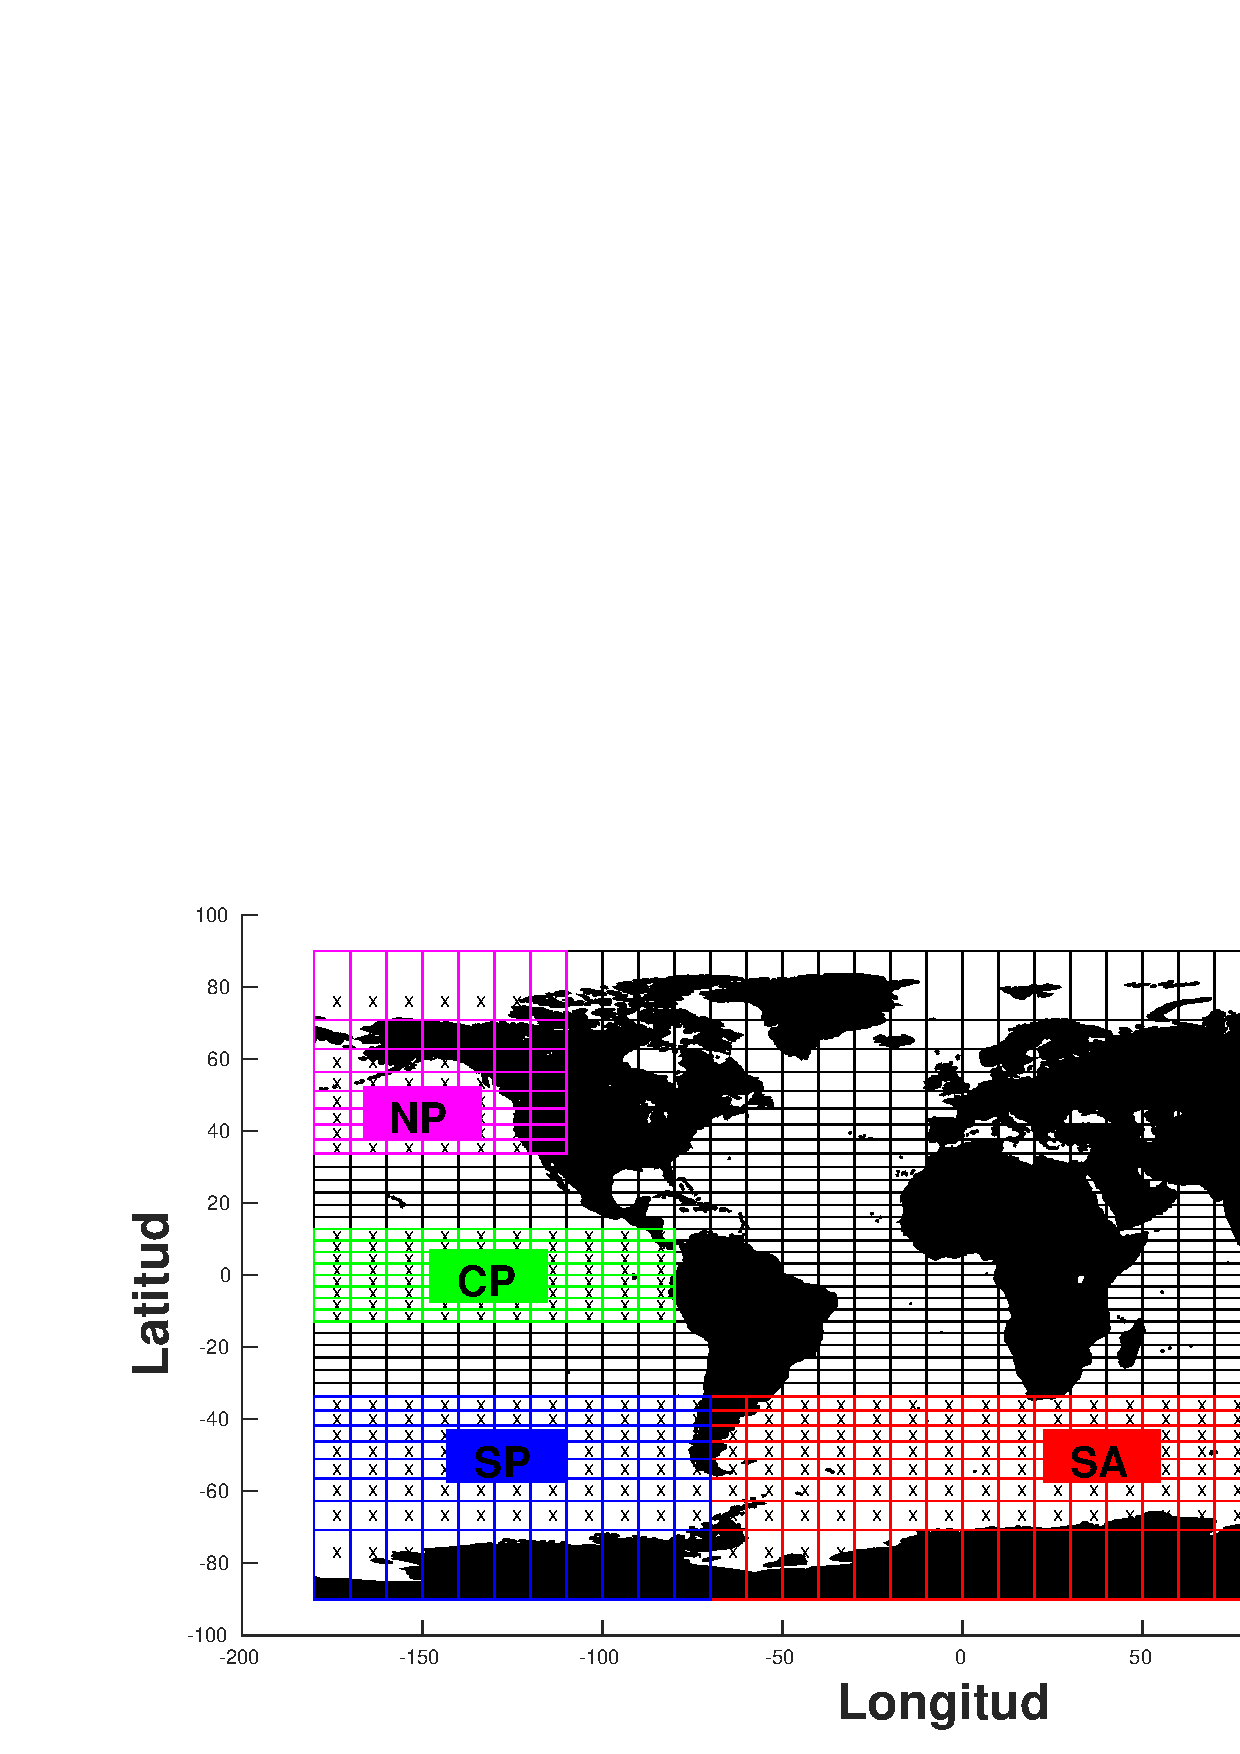
\includegraphics[width=\textwidth]{./imagenes/mapa.png}
   \end{minipage}}  

   \end{center}
\end{frame}
%%%%%%%%%%%%%%%%%%%%%%%%%%%%%%%%%%%%%%%

\begin{frame}{Hipótesis}
\centering
\begin{minipage}[m]{0.9\textwidth}
\begin{alertblock}{\scriptsize{\textit{H}$_0$}} 
  \alert{El polvo no tiene un efecto en el $\Delta$pCO$_{2}$ entre el Holoceno y UMG.} \\
 La variabilidad del pCO$_2$ atmosférico, ha sido consecuencia de mecanismos físicos como la estratificación de los océanos y la temperatura, y equilibrios químicos como la disolución de carbonatos. 

\end{alertblock} \pause
\begin{alertblock}{\scriptsize{\textit{H}$_0$}} 
\alert{El $\Delta$pCO$_{2}$ generado entre el UMG y Holoceno, debido al efecto del polvo, proviene de los cambios en los océanos del sur.} \\
Dada la mayor extención de los océanos del sur se espera tengan un impacto mayor en la variabilidad del pCO$_2$.  
\end{alertblock}
\end{minipage}
\end{frame}

%%%%%%%%%%%%%%%%%%%%%%%%%%%%%%%%%%%%%%%%5
\section{Objetivos}
\begin{frame}{Objetivos}
\begin{alertblock}{}
\begin{enumerate}
\item Cuantificar mediante un modelo biogeoquímico, el nivel de
captura de CO$_2$ por los océanos producto de la bomba biológica orgánica.\pause
\item Calcular la contribución de cada región HNLC a la diferencia de CO$_2$ debido a los distintos flujos de polvo. \pause
\item Determinar la diferencia de CO$_2$ existente entre el UMG y el Holoceno.
  \end{enumerate}
\end{alertblock}

\end{frame}


%%%%%%%%%%%%%%%%%%%%%%%%%%%%%%%%%%
\section{Metodología}

\begin{frame}{Descripción}
\hspace*{-0.05\textwidth}
{
\begin{minipage}[m]{0.375\textwidth}
\only<1-13>{
 \resizebox*{!}{0.85\textheight}{ 
\begin{tikzpicture}[basic/.style={draw, text centered}, node distance = 2.0cm, minimum height=3.5cm, minimum width=1.5cm]
    % Place nodes
    \node [block] (Fp) {\alert<2-4>{Flujos de polvo}};
    \node [cloud, left of=Fp, node distance=3.0cm] (Input) {Input};
    \node [block, below of=Fp] (Regrillado) {\alert<5-7>{Regrillado}};
    \node [cloud, left of=Regrillado, node distance=3.15cm] (Prep) {Preprocesado};
    \node [block, below of=Regrillado] (GNPU) {\alert<5-7>{Generaci\'on de niveles de polvo}};
    \node [blockn, left of=GNPU, node distance=3.0cm] (GNPD) {\alert<8-11>{G. niveles de polvo regionales}};
    \node [block, below of=GNPU] (modelo) {\alert<12>{Modelo cGENIE}};
    \node [cloud, left of=modelo, node distance=3.15cm] (sim) {Simulaciones};
    \node [block, below of=modelo] (Spin) {\alert<13>{spin-up}};
    \node [block, below of=Spin] (Control) {\alert<13>{Control}};
    \node [blockn, below left of=Control, node distance=3cm] (G) {\alert<13>{Globales}};
    \node [blockn, below right of=Control, node distance=3cm] (R) {\alert<13>{Regionales}};

    % Draw edges
    \draw [dashed,->] (Input) -- (Fp);
    \draw [->] (Fp) -- (Regrillado);
    \draw [dashed,->] (Prep) -- (Regrillado);
    \draw [->] (Regrillado) -- (GNPU);
 %%  % \path [line] (Regrillado) |- node [near start] {yes} (GNPU);
    \draw [|->] (GNPU) -- (GNPD);
    \draw [->] (GNPU) -- (modelo);
    \draw [dashed,->] (sim) -- (modelo);
    \draw [->] (modelo) -- (Spin);
    \draw [->] (Spin) -- (Control);
    \draw [|->] (Control) -- (G);
    \draw [|->] (Control) -- (R);

\end{tikzpicture}}%
}
 \only<14>{\centering
   \includegraphics[height=0.3\textheight,width=\textwidth]{./imagenes/Albani_SPIN.png}

\medskip

\centering
   \includegraphics[height=0.35\textheight,width=\textwidth]{./imagenes/HolocenoAlbani.png}}  
\end{minipage}
}
%
{
\hspace*{-15pt}
{
\begin{minipage}[m]{0.6\textwidth}%[t][0.89\textheight]{0.56\textwidth}
  \only<2>{
    \begin{minipage}{\textwidth}
      \begin{block}{\scriptsize{Campos de flujos de polvo}}
        \tiny{Entre la base de datos utilizadas se encuentra una reconstrucción ``Lambert'' \cite{lambert2015dust}, y cuatro modelos de polvo ``MRI-CGCM3'' \cite{yukimoto2012new}, ``MIROC-ESM'' \cite{sueyoshi2013set}, ``Takemura'' \cite{takemura2009simulation}, `Albani'' \cite{albani2014improved}. Todos los campos contienen datos que corresponden al Holoceno y UMG.}
      \end{block}
    \end{minipage}

    \vspace{20pt}

    \begin{minipage}{\textwidth}
      \centering
      {\bf Lambert}
      \medskip

      \hspace*{-0.15\textwidth}
      \includegraphics[width=1.25\textwidth]{./imagenes/Lambert_scale.pdf}
    \end{minipage}
    \vspace{20pt}
  }
  \only<3>{
    \begin{minipage}{\textwidth}
      \centering
      {\bf MRI-CGCM3}
      \medskip

      \hspace*{-0.15\textwidth}
      \includegraphics[width=1.25\textwidth]{./imagenes/MRI-CGCM3_scale.pdf}
      {\bf MIROC-ESM}
      \medskip

      \hspace*{-0.15\textwidth}
      \includegraphics[width=1.25\textwidth]{./imagenes/MIROC-ESM_scale.pdf}
    \end{minipage}
    \vspace{30pt} \,
  }
  \only<4>{
    \begin{minipage}{\textwidth}
      \centering
      {\bf Takemura}
      \medskip

      \hspace*{-0.15\textwidth}
      \includegraphics[width=1.25\textwidth]{./imagenes/Takemura_scale.pdf}
      {\bf Albani}
      \medskip

      \hspace*{-0.15\textwidth}
      \includegraphics[width=1.25\textwidth]{./imagenes/Albani_scale.pdf}
    \end{minipage}
    \vspace{30pt} \,
  }
  \only<5-7>{
    \centering
    \uncover<5-7>{
      \begin{block}{Preprocesamiento}
        \begin{itemize}
        \item{}\scriptsize{ Los campos de flujos de polvo fueron traspazados a una dimensión de 36x36 puntos de grilla.}
        \item{}\scriptsize{ Se realizó una interpolación equiespaciada, creando con ello 8 diferentes escenarios intermedios de polvo. Éstos en conjunto con el item 1 generan 10 niveles que van desde el Holoceno hasta el UMG incluyendo ambos periodos. }
        \end{itemize}
      \end{block}
    }
    \vspace{1cm}
    \uncover<5-7>{
      \hspace{10pt}
      \begin{minipage}[m]{0.225\textwidth}
      \hspace*{-10pt}\includestandalone[width=0.95\textwidth]{./tikz/cuadrado}
      \end{minipage}
    }
    \uncover<6-7>{
      \hspace{-25pt}
      \begin{minipage}[m]{0.04\textwidth}      
      \includestandalone[width=0.95\textwidth]{./tikz/flecha}
      \end{minipage}
      \hspace{-10pt}
    } 
    \uncover<6-7>{
      \begin{minipage}[m]{0.225\textwidth}
      \includestandalone[width=0.95\textwidth]{./tikz/cuadrado2_2}
      \end{minipage} 
    } 
    \uncover<7>{
      \hspace{-10pt}
      \begin{minipage}[m]{0.04\textwidth}
      \includestandalone[width=0.95\textwidth]{./tikz/flecha}
      \end{minipage}
      \begin{minipage}[m]{0.04\textwidth} 
      \includestandalone[width=0.95\textwidth]{./tikz/puntos}
      \end{minipage}
      \begin{minipage}[m]{0.04\textwidth}       
      \includestandalone[width=0.95\textwidth]{./tikz/flecha}
      \end{minipage}
      \hspace{-10pt}
    } 
    \uncover<5-7>{
      \begin{minipage}[m]{0.225\textwidth}
      \includestandalone[width=0.95\textwidth]{./tikz/cuadrado10}
      \end{minipage}
    }    
  }
  \only<8-11>{
    \centering
    \uncover<8-11>{
      \begin{block}{Preprocesamiento}
        \begin{itemize}
          \item \scriptsize{Se generaron nuevos campos de polvo regionales, a partir de los 10 producidos de la combinación del item 1 e item 2.}
        \end{itemize}
      \end{block}
    }
    \vspace{1cm}
    \uncover<8-11>{
      \begin{minipage}[m]{0.225\textwidth}
      \hspace*{-10pt}\includestandalone[width=0.95\textwidth]{./tikz/cuadrado1}
      \end{minipage}
    }
    \uncover<9-11>{
      \hspace{-25pt}
      \begin{minipage}[m]{0.04\textwidth}      
      \includestandalone[width=0.95\textwidth]{./tikz/flecha}
      \end{minipage}
      \hspace{-10pt}
    } 
    \uncover<9-11>{
      \begin{minipage}[m]{0.225\textwidth}
      \includestandalone[width=0.95\textwidth]{./tikz/cuadrado2}
      \end{minipage} 
    } 
    \uncover<10-11>{
      \hspace{-10pt}
      \begin{minipage}[m]{0.04\textwidth}
      \includestandalone[width=0.95\textwidth]{./tikz/flecha}
      \end{minipage}
      \begin{minipage}[m]{0.04\textwidth} 
      \includestandalone[width=0.95\textwidth]{./tikz/puntos}
      \end{minipage}
      \begin{minipage}[m]{0.04\textwidth}       
      \includestandalone[width=0.95\textwidth]{./tikz/flecha}
      \end{minipage}
      \hspace{-10pt} 
    } 
    \uncover<11-11>{
      \begin{minipage}[m]{0.225\textwidth}
      \includestandalone[width=0.95\textwidth]{./tikz/cuadrado3}
      \end{minipage}
    }
  }  
  \only<12>{
  \centering
  \begin{block}{Procesamiento}
  %\begin{itemize}
  \scriptsize{Se utilizó un código versión “muffin” del \alert{\textit{cGENIE Earth system Model
  of Intermediate Complexity}} \cite{ridgwell2007regulation}. Los módulos utilizados fueron:}
  \begin{itemize}
    \item{} \scriptsize{Atmósfera (EMBM 2D)}
    \item{} \scriptsize{Océano/cubierta de hielo (GOLDSTEIN)}
    \item{} \scriptsize{Química Atmosférica (ATCHEM)}
    \item{} \scriptsize{Biogeoquímica oceánica (BIOGEM)}
    \end{itemize} 
  %\end{itemize}
  \end{block}

  \centering
      \includegraphics[width=0.7\textwidth,height=0.35\textheight]{./imagenes/Parekh.png}
  }
\only<13-14>{\hspace*{-0.025\textwidth}
   \centering
   
\includegraphics[width=0.99\textwidth]{./imagenes/runcGENIE2.pdf}
  \hspace{10pt}
  \begin{minipage}[m]{0.9\textwidth}
    \begin{block}{Procesamiento}
      \tiny{Todas las corridas tuvieron 10000 iteraciones. }
      \begin{itemize}
        \item{} \tiny{Validación: spin-up, CO$_2$ fijo en 278 (periodo preindustrial)}
        \item{} \tiny{Validación: control, CO$_2$ libre, concentración de polvo periodo preindustrial} 
        \item{} \tiny{Simulación: Globales, CO$_2$ libre, niveles de polvo globales del 2 al 10}
        \item{} \tiny{Simulación: Regionales, CO$_2$ libre, niveles de polvo zonas HNLC del 2 al 10}
      \end{itemize}
    \end{block} 
  \end{minipage}
  \vspace{0.5cm}
  }    
%%%    
\end{minipage}
}
}
\end{frame}
%%%%%%%%%%%%%%%%%%%%%%%%%%%%%%%%%%%%%%%%%%%%%%%

\section{Resultados}

\begin{frame}
\frametitle{Resultados}
\framesubtitle{Globales}
\centering
\vspace{-20pt}
\begin{minipage}[t][0.2\textheight][t]{\textwidth}
  \begin{block}{}
  \begin{itemize}
    \item{} \scriptsize{La simulación Albani y MIROC-ESM muestran el mayor $\Delta$pCO$_2$ (21.6 y 20.3 ppm).
    \item{} Lambert tiene los más elevados y mayores $\Delta$ de flujo de polvo (16 ppm). 
    \item{} MRI-CGCM3 presenta la menor reducción de pCO$_2$ (9 ppm).}
  \end{itemize}
  \end{block}
\end{minipage}

\vspace{20pt}

{
\begin{minipage}{0.6\textwidth}
\pgfplotstableread{./plot/Datos_ppm_All.dat}
\table
\begin{tikzpicture}[scale=0.75]
\begin{axis}[
        axis y line=left,  
        y axis line style=blue!75!black,  
   % title={bla}
    xlabel={Niveles de polvo},
    ylabel={Concentración de pCO$_2$ (ppm)},
    xmin=1, xmax=10,
   ymin=256, ymax=278.5,
    xtick={2,4,6,8,10},
    %ytick={310,320,330,340,350,360,370,380,390,400},
    legend pos=north west,
    ymajorgrids=true,
    grid style=dashed, 
] 
\addplot[
   color=green,
   mark=square,
    ] table[y=Lambert] from \table;
 %\addlegendentry{Lambert}

 \addplot[
   color=black,
   mark=square,
    ] table[y=MRI_CGCM3] from \table;
 %\addlegendentry{MRI-CGCM3}

 \addplot[
   color=pink,
   mark=square,
    ] table[y=MIROC_ESM] from \table;
 %\addlegendentry{MIROC-ESM}

\addplot[
   color=blue,
   mark=square,
    ] table[y=Takemura] from \table;
 %\addlegendentry{Takemura}

 \addplot[
   color=red,
   mark=square,
    ] table[y=Albani] from \table;            
  % \addlegendentry{Albani}

   \end{axis}
\pgfplotstableread{./plot/Rest_CO2_All2.dat}
\tabla
\begin{axis}[
        axis y line=right,
        ylabel=$\Delta$pCO$_2$ (ppm),
        y axis line style=red!75!black,
        axis x line=none,
        ]
  \addplot[
   color=green,
   mark=*,
   dashed,
    ] table[y=Modelo_Lambert] from \tabla;
 %\addlegendentry{Lambert}

 \addplot[
   color=black,
      mark=*,
   dashed,
    ] table[y=Modelo_MRI_CGCM3] from \tabla;
 %\addlegendentry{MRI-CGCM3}

 \addplot[
   color=pink,
      mark=*,
   dashed,
    ] table[y=Modelo_MIROC-ESM] from \tabla;
 %\addlegendentry{MIROC-ESM}

\addplot[
   color=blue,
      mark=*,
   dashed,
    ] table[y=Modelo_Takemura] from \tabla;
 %\addlegendentry{Takemura}

 \addplot[
   color=red,
   mark=*,
   dashed,
    ] table[y=Modelo_Albani] from \tabla;            
 %\addlegendentry{Lambert}
    \end{axis}
\end{tikzpicture}
\end{minipage}}
\quad
\begin{minipage}[m]{0.2\textwidth}
  \begin{flushleft}
  \tiny
  Leyenda 

  Concentración de pCO$_2$ (ppm)
  \includestandalone[width=\textwidth]{./tikz/legend}
  $\Delta$pCO$_2$ (ppm)
  \includestandalone[width=\textwidth]{./tikz/legend2}
  \end{flushleft}
\end{minipage}

\end{frame}


\begin{frame}
\frametitle{Resultados}
\framesubtitle{Pacífico Norte (NP)}
\centering
\vspace{-20pt}
\begin{minipage}[t][0.2\textheight][t]{\textwidth}
  \begin{block}{}
  \begin{itemize}
    \item{} \scriptsize{ Albani estimó la mayor reducción de CO$_2$ hacia el UMG (7 ppm). 
    \item{} Lambert posee mayores flujos de polvo que Albani, pero estima menor concentración de pCO$_2$ (5 ppm) que MIROC-ESM (5.53 ppm). 
    \item{} Takemura tiene la más baja estimación de pCO$_2$ (1.14 ppm).}
  \end{itemize}
  \end{block}
\end{minipage}

\vspace{20pt}


\begin{minipage}{0.6\textwidth}
\pgfplotstableread{./plot/Datos_ppm_NP.dat}
\tablaNP
\begin{tikzpicture}[scale=0.75]
\begin{axis}[
        axis y line=left,  
        y axis line style=blue!75!black,  
   % title={bla}
    xlabel={Niveles de polvo},
    ylabel={Concentración de pCO$_2$ (ppm)},
    xmin=1, xmax=10,
   ymin=271, ymax=278.5,
 %   xtick={1950,1960,1970,1980,1990,2000,2010},
 %   ytick={310,320,330,340,350,360,370,380,390,400},
    legend pos=north west,
    ymajorgrids=true,
    grid style=dashed, 
] 
\addplot[
   color=green,
   mark=square,
    ] table[y=Lambert] from \tablaNP;

 \addplot[
   color=black,
   mark=square,
    ] table[y=MRI_CGCM3] from \tablaNP;

 \addplot[
   color=pink,
   mark=square,
    ] table[y=MIROC_ESM] from \tablaNP;

\addplot[
   color=blue,
   mark=square,
    ] table[y=Takemura] from \tablaNP;

 \addplot[
   color=red,
   mark=square,
    ] table[y=Albani] from \tablaNP;            
 %  \legend{CuSO$_4\cdot$5H$_2$O}
   \end{axis}
\pgfplotstableread{./plot/Rest_CO2_NP2.dat}
\tableNP
\begin{axis}[
        axis y line=right,
        ylabel=$\Delta$pCO$_2$ (ppm),
        y axis line style=red!75!black,
        axis x line=none,
        ]
  \addplot[
   color=green,
   mark=*,
   dashed,
    ] table[y=Modelo_Lambert] from \tableNP;

 \addplot[
   color=black,
      mark=*,
   dashed,
    ] table[y=Modelo_MRI_CGCM3] from \tableNP;

 \addplot[
   color=pink,
      mark=*,
   dashed,
    ] table[y=Modelo_MIROC-ESM] from \tableNP;

\addplot[
   color=blue,
      mark=*,
   dashed,
    ] table[y=Modelo_Takemura] from \tableNP;

 \addplot[
   color=red,
   mark=*,
   dashed,
    ] table[y=Modelo_Albani] from \tableNP;            
 %  \legend{CuSO$_4\cdot$5H$_2$O}
    \end{axis}

\end{tikzpicture}
\end{minipage}
\quad
\begin{minipage}[m]{0.2\textwidth}
  \begin{flushleft}
  \tiny
  Leyenda 

  Concentración de pCO$_2$ (ppm)
  \includestandalone[width=\textwidth]{./tikz/legend}
  $\Delta$pCO$_2$ (ppm)
  \includestandalone[width=\textwidth]{./tikz/legend2}
  \end{flushleft}
\end{minipage}

\end{frame}


%------------------------------------------------------%
\begin{frame}
\frametitle{Resultados}
\framesubtitle{Pacífico Central (CP)}
\centering
\vspace{-20pt}
\begin{minipage}[t][0.2\textheight][t]{\textwidth}
  \begin{block}{}
  \begin{itemize}
    \item{} \scriptsize{ Los valores de pCO$_2$ son bajos y similares. 
    \item{} El mayor aporte a la reducción es MIROC-ESM (3.6 ppm). 
    \item{} MRI-CGCM3 posee la más baja reducción con $\sim$ 0.8 ppm}
  \end{itemize}
  \end{block}
\end{minipage}

\vspace{20pt}


\begin{minipage}{0.6\textwidth}
\pgfplotstableread{./plot/Datos_ppm_CP.dat}
\tablaCP
\begin{tikzpicture}[scale=0.75]
\begin{axis}[
        axis y line=left,  
        y axis line style=blue!75!black,  
   % title={bla}
    xlabel={Niveles de polvo},
    ylabel={Concentración de pCO$_2$ (ppm)},
    xmin=1, xmax=10,
   ymin=274, ymax=278.5, %   xtick={1950,1960,1970,1980,1990,2000,2010},
 %   ytick={310,320,330,340,350,360,370,380,390,400},
    legend pos=north west,
    ymajorgrids=true,
    grid style=dashed, 
] 
\addplot[
   color=green,
   mark=square,
    ] table[y=Lambert] from \tablaCP;

 \addplot[
   color=black,
   mark=square,
    ] table[y=MRI_CGCM3] from \tablaCP;

 \addplot[
   color=pink,
   mark=square,
    ] table[y=MIROC_ESM] from \tablaCP;

\addplot[
   color=blue,
   mark=square,
    ] table[y=Takemura] from \tablaCP;

 \addplot[
   color=red,
   mark=square,
    ] table[y=Albani] from \tablaCP;            
 %  \legend{CuSO$_4\cdot$5H$_2$O}
   \end{axis}
\pgfplotstableread{./plot/Rest_CO2_CP2.dat}
\tableCP
\begin{axis}[
        axis y line=right,
        ylabel=$\Delta$pCO$_2$ (ppm),
        y axis line style=red!75!black,
        axis x line=none,
        ]
  \addplot[
   color=green,
   mark=*,
   dashed,
    ] table[y=Modelo_Lambert] from \tableCP;

 \addplot[
   color=black,
      mark=*,
   dashed,
    ] table[y=Modelo_MRI_CGCM3] from \tableCP;

 \addplot[
   color=pink,
      mark=*,
   dashed,
    ] table[y=Modelo_MIROC-ESM] from \tableCP;

\addplot[
   color=blue,
      mark=*,
   dashed,
    ] table[y=Modelo_Takemura] from \tableCP;

 \addplot[
   color=red,
   mark=*,
   dashed,
    ] table[y=Modelo_Albani] from \tableCP;            
 %  \legend{CuSO$_4\cdot$5H$_2$O}
    \end{axis}
\end{tikzpicture}
\end{minipage}
\quad
\begin{minipage}[m]{0.2\textwidth}
  \begin{flushleft}
  \tiny
  Leyenda 

  Concentración de pCO$_2$ (ppm)
  \includestandalone[width=\textwidth]{./tikz/legend}
  $\Delta$pCO$_2$ (ppm)
  \includestandalone[width=\textwidth]{./tikz/legend2}
  \end{flushleft}
\end{minipage}

\end{frame}



\begin{frame}
\frametitle{Resultados}
\framesubtitle{Pacífico Sur (SP)}
\centering
\vspace{-20pt}
\begin{minipage}[t][0.2\textheight][t]{\textwidth}
  \begin{block}{}
  \begin{itemize}
    \item{} \scriptsize{Lambert tiene una disminución mayor de CO$_2$ para el UMG de 4.6 ppm.  
    \item{} Takemura muestra un ínfima reducción de pCO$_2$ ($\sim$ 0.04 ppm).
    \item{} MRI-CGCM3 y MIROC-ESM no tienen fuentes de polvo en esta zona. } 
  \end{itemize}
  \end{block}
\end{minipage}

\vspace{20pt}


\begin{minipage}{0.6\textwidth}
\pgfplotstableread{./plot/Datos_ppm_SP.dat}
\tablaSP
\begin{tikzpicture}[scale=0.75]
\begin{axis}[
        axis y line=left,  
        y axis line style=blue!75!black,  
   % title={bla}
    xlabel={Niveles de polvo},
    ylabel={Concentración de pCO$_2$ (ppm)},
    xmin=1, xmax=10,
   ymin=265, ymax=278.5,
 %   xtick={1950,1960,1970,1980,1990,2000,2010},
 %   ytick={310,320,330,340,350,360,370,380,390,400},
    legend pos=north west,
    ymajorgrids=true,
    grid style=dashed, 
] 
\addplot[
   color=green,
   mark=square,
    ] table[y=Lambert] from \tablaSP;

 \addplot[
   color=black,
   mark=square,
    ] table[y=MRI_CGCM3] from \tablaSP;

 \addplot[
   color=pink,
   mark=square,
    ] table[y=MIROC_ESM] from \tablaSP;

\addplot[
   color=blue,
   mark=square,
    ] table[y=Takemura] from \tablaSP;

 \addplot[
   color=red,
   mark=square,
    ] table[y=Albani] from \tablaSP;            
 %  \legend{CuSO$_4\cdot$5H$_2$O}
   \end{axis}
\pgfplotstableread{./plot/Rest_CO2_SP2.dat}
\tableSP
\begin{axis}[
        axis y line=right,
        ylabel=$\Delta$pCO$_2$ (ppm),
        y axis line style=red!75!black,
        axis x line=none,
        ]
  \addplot[
   color=green,
   mark=*,
   dashed,
    ] table[y=Modelo_Lambert] from \tableSP;

 \addplot[
   color=black,
      mark=*,
   dashed,
    ] table[y=Modelo_MRI_CGCM3] from \tableSP;

 \addplot[
   color=pink,
      mark=*,
   dashed,
    ] table[y=Modelo_MIROC-ESM] from \tableSP;

\addplot[
   color=blue,
      mark=*,
   dashed,
    ] table[y=Modelo_Takemura] from \tableSP;

 \addplot[
   color=red,
   mark=*,
   dashed,
    ] table[y=Modelo_Albani] from \tableSP;            
 %  \legend{CuSO$_4\cdot$5H$_2$O}
    \end{axis}
\end{tikzpicture}
\end{minipage}
\quad
\begin{minipage}[m]{0.2\textwidth}
  \begin{flushleft}
  \tiny
  Leyenda 

  Concentración de pCO$_2$ (ppm)
  \includestandalone[width=\textwidth]{./tikz/legend}
  $\Delta$pCO$_2$ (ppm)
  \includestandalone[width=\textwidth]{./tikz/legend2}
  \end{flushleft}
\end{minipage}

\end{frame}


\begin{frame}
\frametitle{Resultados}
\framesubtitle{Atlántico/Índico Sur (SAI)}
\centering
\vspace{-20pt}
\begin{minipage}[t][0.2\textheight][t]{\textwidth}
  \begin{block}{}
  \begin{itemize}
    \item{} \scriptsize{Albani estima la mayor reducción de pCO$_2$ para el UMG (12.5). } 
    \item{} Lambert calcula una reducción de 6 ppm. 
    \item{} Takemura y MIROC-ESM no poseen fuentes de polvo en la región. 
  \end{itemize}
  \end{block}
\end{minipage}

\vspace{20pt}


\begin{minipage}{0.6\textwidth}
\pgfplotstableread{./plot/Datos_ppm_SA.dat}
\tablaSA
\begin{tikzpicture}[scale=0.75]
\begin{axis}[
        axis y line=left,  
        y axis line style=blue!75!black,  
   % title={bla}
    xlabel={Niveles de polvo},
    ylabel={Concentración de pCO$_2$ (ppm)},
    xmin=1, xmax=10,
   ymin=265, ymax=279.5,
 %   xtick={1950,1960,1970,1980,1990,2000,2010},
 %   ytick={310,320,330,340,350,360,370,380,390,400},
    legend pos=north west,
    ymajorgrids=true,
    grid style=dashed, 
] 
\addplot[
   color=green,
   mark=square,
    ] table[y=Lambert] from \tablaSA;

 \addplot[
   color=black,
   mark=square,
    ] table[y=MRI_CGCM3] from \tablaSA;

 \addplot[
   color=pink,
   mark=square,
    ] table[y=MIROC_ESM] from \tablaSA;

\addplot[
   color=blue,
   mark=square,
    ] table[y=Takemura] from \tablaSA;

 \addplot[
   color=red,
   mark=square,
    ] table[y=Albani] from \tablaSA;            
 %  \legend{CuSO$_4\cdot$5H$_2$O}
   \end{axis}
\pgfplotstableread{./plot/Rest_CO2_SA2.dat}
\tableSA
\begin{axis}[
        axis y line=right,
        ylabel=$\Delta$pCO$_2$ (ppm),
        y axis line style=red!75!black,
        axis x line=none,
        ]
  \addplot[
   color=green,
   mark=*,
   dashed,
    ] table[y=Modelo_Lambert] from \tableSA;

 \addplot[
   color=black,
      mark=*,
   dashed,
    ] table[y=Modelo_MRI_CGCM3] from \tableSA;

 \addplot[
   color=pink,
      mark=*,
   dashed,
    ] table[y=Modelo_MIROC-ESM] from \tableSA;

\addplot[
   color=blue,
      mark=*,
   dashed,
    ] table[y=Modelo_Takemura] from \tableSA;

 \addplot[
   color=red,
   mark=*,
   dashed,
    ] table[y=Modelo_Albani] from \tableSA;            
 %  \legend{CuSO$_4\cdot$5H$_2$O}
    \end{axis}

\end{tikzpicture}
\end{minipage}
\quad
\begin{minipage}[m]{0.2\textwidth}
  \begin{flushleft}
  \tiny
  Leyenda 

  Concentración de pCO$_2$ (ppm)
  \includestandalone[width=\textwidth]{./tikz/legend}
  $\Delta$pCO$_2$ (ppm)
  \includestandalone[width=\textwidth]{./tikz/legend2}
  \end{flushleft}
\end{minipage}

\end{frame}




\begin{frame}
\frametitle{Resultados}
\framesubtitle{}
\begin{center}
\includegraphics[width=0.8\textwidth]{./imagenes/Ponderaciones_LGM.png}
\vspace{1cm}

\begin{minipage}[b][0.2\textheight][b]{\textwidth}
 
  \begin{block}{}
  \begin{itemize}
    \item{} \scriptsize{ La zona NP contribuye en promedio en un $\sim$ 24$\%$  (4.2 ppm). 
    \item{} La región CP aporta en promedio 16$\%$ (2 ppm) del valor total.
    \item{} La zona SP en promedio disminuye el pCO$_2$ en un $\sim$ 14$\%$ (1.5 pmm). 
    \item{} La región SAI reduce la concentración de pCO$_2$ en 46$\%$ (3.5 ppm) .}
  \end{itemize}
  \end{block}
\end{minipage}

\end{center}
\end{frame}

%%%%%%%%%%%%%%%%%%%%%%%%%%%%%%%%%%%%%%%

\section{Consideraciones finales}
\begin{frame}{Consideraciones finales}


\only<1>{\begin{minipage}[t][0.3\textheight][t]{\textwidth}
\begin{alertblock}{}
\begin{itemize}
  \item{} \scriptsize{ Se rechaza la $H_{0}$ (1) dado que el polvo se comprobó actúa como forzante del ciclo del carbono. 
  \item{} La máxima reducción de pCO$_2$ a nivel global fue en promedio de $\sim$ 16 ppm.
  \item{} Se rechaza la $H_{0}$ (2). En general todas las cuencas oceánicas juegan un rol en la captura de CO$_2$, particularmente este efecto se refleja en las zonas HNLC.}

\end{itemize}
\end{alertblock} 
\end{minipage}}

\only<2>{\begin{minipage}[t][0.3\textheight][t]{\textwidth}
\begin{alertblock}{}
 \begin{itemize} 

  \item{} \scriptsize{Los resultados presentados están sujetos a la variabilidad inducida por los propios campos de polvo utilizados en cGENIE.  
  \item{} La mayor liberación de polvo habría permitido mejorar la utilización del NO$^{-}_{3}$ y PO$^{3-}_{4}$ dejando un excedente de Si(OH)$_{4}$.  
  \item{} Existen otro mecanismos que podrían estar participando en la diferencia de entre 80 y 100 ppm de CO$_2$, por ejemplo, estratificación de los océanos, temperatura, disolución de carbonatos. }

\end{itemize}
\end{alertblock}
\end{minipage}} 


\uncover<1-2>{\begin{center}
\resizebox{12cm}{!} {%

\begin{tabular}{|c||c|c||c|c||c|c||c|c||c|c|}
\hline
\multirow{2}{*}{\bf Zona/Modelo} & \multicolumn{2}{c}{\bf Albani} & \multicolumn{2}{c}{\bf Lambert} & \multicolumn{2}{c}{\bf Takemura} & \multicolumn{2}{c}{\bf MIROC-ESM} & \multicolumn{2}{c}{\bf MRI-CGCM3} \\ \cline{2-11} 
 & Máx. & Min. & Máx. & Min.& Máx. & Min.& Máx. & Min.& Máx. & Min.\\ \hline \hline
{\bf Global} & 278.07 & 256.44 & 278.09 & 261.50 & 278.09 & 262.10 & 278.08& 257.78 & 278.07 & 269.15 \\ \hline
{ \bf Pacífico norte} & 278.07 & 271.11& 278.09 & 273.00& 278.09 & 276.94 & 278.08 & 272.55 & 278.07 & 275.57\\ \hline
{\bf Pacífico central} & 278.07 &277.39 & 278.09 & 275.70& 278.09 &275.52 & 278.08 & 274.47& 278.07 &277.30 \\ \hline
{\bf Pacífico sur} & 278.07 & 275.02& 278.09 &273.52 & 278.09 &278.04 & 278.14 & 278.08& 278.18 & 278.07 \\ \hline
{\bf Atlántico/Índico sur} & 278.07 & 265.54& 278.09 &272.42 & 278.58 &278.09 & 279.31 &278.08 & 278.07 &277.03 \\ \hline \hline

\end{tabular}}
\end{center}}

\end{frame}
%%%%%%%%%%%%%%%%%%%%%%%%%%%%%%%%
  
\begin{frame}[t,allowframebreaks]
  \frametitle{References}
  \printbibliography[heading=subbibliography  ,title={References}]
 \end{frame}
%%%%%%%%%%%%%%%%%%%%%%%%%%%%%%%%
\begin{frame}{}
\begin{center}
\Huge
Gracias :)
\end{center}
\end{frame}
\end{document}
